% 来源：固定1991上海PDF第1页（印刷5-33），第14题四幅选项图。
% 仅忠实复现原图的定性曲线与坐标轴，不假设尚未辨清的题面指数。
% 贝塞尔控制点是绘图参数，不是原题给出的函数值或坐标条件。
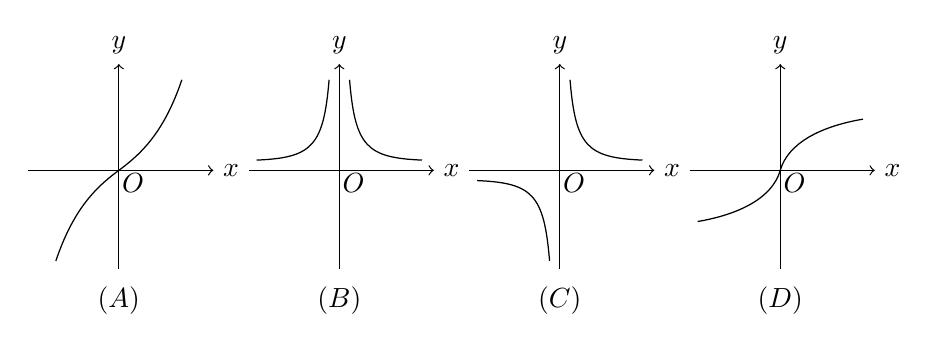
\begin{tikzpicture}[line width=0.45pt,scale=1.0]
  \foreach \offset/\choice in {0/A,2.8/B,5.6/C,8.4/D}{
    \begin{scope}[xshift=\offset cm]
      \draw[->] (-1.15,0)--(1.2,0) node[right] {$x$};
      \draw[->] (0,-1.25)--(0,1.35) node[above] {$y$};
      \node[below right,inner sep=1pt] at (0,0) {$O$};
      \node at (0,-1.65) {$(\choice)$};
    \end{scope}
  }
  \draw (-0.8,-1.15) .. controls (-0.58,-0.5) and (-0.3,-0.22) .. (0,0)
    .. controls (0.3,0.22) and (0.58,0.5) .. (0.8,1.15);
  \begin{scope}[xshift=2.8cm]
    \draw (-1.05,0.13) .. controls (-0.35,0.16) and (-0.2,0.3) .. (-0.13,1.15);
    \draw (0.13,1.15) .. controls (0.2,0.3) and (0.35,0.16) .. (1.05,0.13);
  \end{scope}
  \begin{scope}[xshift=5.6cm]
    \draw (-1.05,-0.13) .. controls (-0.35,-0.16) and (-0.2,-0.3) .. (-0.13,-1.15);
    \draw (0.13,1.15) .. controls (0.2,0.3) and (0.35,0.16) .. (1.05,0.13);
  \end{scope}
  \begin{scope}[xshift=8.4cm]
    \draw (-1.05,-0.65) .. controls (-0.52,-0.56) and (-0.1,-0.35) .. (0,0)
      .. controls (0.1,0.35) and (0.52,0.56) .. (1.05,0.65);
  \end{scope}
\end{tikzpicture}
